%!TEX root = ../main.tex

\chapter{Teoria dei giochi}
\label{cha:teoria_dei_giochi}

La \textbf{teoria dei giochi} analizza situazioni in cui vi sono interazioni tra \textbf{agenti} diversi, ove ognuno è interessato a \textbf{massimizzare} il proprio \textbf{beneficio}, tali per cui le scelte di un agente possono influire sul beneficio che possono ottenere gli altri agenti. Essa è stata sviluppata con il preciso scopo di sopperire alle limitazioni legate all'ottimizzazione di una \textbf{singola} funzione obiettivo.

Vediamo brevemente gli avvenimenti più importanti nello studio della teoria dei giochi:
\begin{itemize}
	\item \textbf{1921 - 1928}: prima formulazione di strategia mista e l'idea di trovare soluzioni di giochi in forma normale (E. Borel, J. von Neumann);
	\item \textbf{1944, 1947}: pubblicazione di 	\emph{Theory of Games and Economic Behavior} (J. von Neumann, O. Morgenstern);
	\item \textbf{1950 - 1953}: contributi alla teoria dei giochi non cooperativi (J. Nash);
	\item \textbf{1972 - 1982}: applicazione della teoria dei giochi a problemi biologici (J. M. Smith).
\end{itemize}

\section{Giochi finiti in forma normale}
\label{sec:giochi_finiti_in_forma_normale}

Un gioco finito in forma normale consiste di un insieme di \textbf{giocatori}
\begin{displaymath}
	I = \{1, \dots, n\} \qquad (n \geq 2)
\end{displaymath}
ciascuno dei quali ha a disposizione un insieme di \textbf{azioni} (dette anche \textbf{strategie pure}):
\begin{displaymath}
	S_i = \{1, \dots, m_i\} \qquad (m_i \geq 2)
\end{displaymath}
L'insieme delle azioni giocate dagli individui in un dato istante prende il nome di \textbf{profilo strategico puro}
\begin{displaymath}
	\vec{s} = (s_1, \dots, s_n)
\end{displaymath}
e l'insieme dei profili strategici puri forma lo \textbf{spazio delle strategie pure}:
\begin{displaymath}
	S = \prod_{i = 1}^n S_i
\end{displaymath}
In seguito alla giocata di un profilo strategico $\vec{s} \in S$ ciascun individuo $i \in I$ ottiene un \textbf{payoff}, ovvero la quantificazione del beneficio ottenuto dal giocatore in seguito alla giocata. Il payoff del giocatore $i$ è rappresentato dalla funzione $\pi_i: S \rightarrow \mathbb{R}$; la \textbf{funzione di payoff combinata} $\vec{\pi}: S \rightarrow \mathbb{R}^n$ assegna ad ogni profilo strategico $\vec{s} \in S$ il vettore
\begin{displaymath}
	\vec{\pi}(\vec{s}) = (\pi_1(\vec{s}), \dots, \pi_n(\vec{s}))
\end{displaymath}
Un gioco in forma normale può dunque essere rappresentato dalla tripletta $(I, S, \vec{\pi})$.

\section{Giochi a due giocatori}

Nel caso speciale di giochi a due giocatori, è comodo rappresentare le funzioni di payoff in forma matriciale:
\begin{itemize}
	\item $\mat{A} = (a_{ij})$ è la matrice di payoff del primo giocatore, dove $a_{ij} = \pi_1(i, j)$ con $i \in S_1, j \in S_2$;
	\item $\mat{B} = (b_{ij})$ è la matrice di payoff del secondo giocatore, dove $b_{ij} = \pi_2(i, j)$ con $i \in S_1, j \in S_2$;
\end{itemize}
In base alle caratteristiche di $\mat{A}$ e $\mat{B}$ si possono distinguere delle categorie particolari di giochi:
\begin{itemize}
	\item \textbf{giochi a somma zero}: $\mat{A} + \mat{B} = \mat{0}$;
	\item \textbf{giochi simmetrici}: $\mat{A} = \mat{B}^T$;
	\item \textbf{giochi doppiamente simmetrici}: $\mat{A} = \mat{A}^T = \mat{B}^T$.
\end{itemize}

\section{Giochi succinti}

Per descrivere un gioco in forma normale, con $n$ giocatori e $m$ strategie pure per ciascuno, occorre memorizzare $n m^n$ numeri. Un \textbf{gioco succinto} è un gioco rappresentabile in forma molto più ridotta rispetto alla forma normale; ad esempio:
\begin{itemize}
	\item \textbf{giochi sparsi}, dove la maggior parte dei payoff è $0$;
	\item \textbf{giochi grafici}, dove i payoff di un giocatore dipendono dalle scelte di $d < n$ giocatori;
	\item \textbf{giochi simmetrici}.
\end{itemize}

\section{Polymatrix games}

Un \textbf{polymatrix game} è un gioco non cooperativo\footnote{Un gioco si dice \textbf{non cooperativo} se non c'è collaborazione tra i giocatori: tutti i giochi che tratteremo sono di questo tipo.} succinto in cui l'influenza relativa della scelta di una strategia da parte di un giocatore sul payoff di un altro è sempre la stessa, indipendentemente da cosa faranno i rimanenti giocatori. Formalmente:
\begin{itemize}
	\item ci sono $n$ giocatori con $m$ strategie pure ciascuno;
	\item c'è una matrice di payoff $A^{ij} = (a_{kl}^{ij})$ di dimensione $m \times m$ per ogni coppia di giocatori $(i, j)$;
	\item il payoff del giocatore $i$ per il profilo strategico puro $\vec{s}$ è:
	\begin{displaymath}
		u_i(\vec{s}) = \sum_{j \neq i} a_{s_i s_j}^{ij}
	\end{displaymath}
\end{itemize}
Il numero di payoff da memorizzare è $\mathcal{O}(m^2 n^2)$. Il problema di trovare un equilibrio di Nash in un gioco di questo tipo è PPAD-completo.\footnote{PPAD è un sottoinsieme di TFNP, un'estensione della classe di problemi decisionali NP a relazioni totali. Una relazione binaria $P \in TFNP$ se e solo se esiste un algoritmo che può verificare in tempo polinomiale se, dati $x$ e $y$, $P(x, y)$ è verificata e $\forall x \exists y$ tale che $P(x, y)$ vale.}

\section{Strategie miste}

Supponiamo che il giocatore $i \in I$ decida la strategia pura da usare in base ad una distribuzione di probabilità sull'insieme di strategie pure $S_i$: tale distribuzione prende il nome di \textbf{strategia mista}. Essa può essere rappresentata da un vettore $m_i$-dimensionale $\vec{x}_i$ dove $x_{ih}$ è la probabilità che il giocatore $i$ giochi la sua strategia pura $h$. Per definizione di distribuzione di probabilità, $\vec{x}_i$ appartiene al simplesso standard $m_i$-dimensionale $\Delta_i$:
\begin{displaymath}
	\Delta_i = \left\{ \vec{x}_i \in \R^{m_i} : \sum_{h = 1}^{m_i} x_{ih} = 1 \text{ e } x_{ih} \geq 0 \; \forall h \right\}
\end{displaymath}
L'insieme delle strategie pure cui è assegnata una probabilità positiva prende il nome di \textbf{supporto} di $\vec{x_i}$:
\begin{displaymath}
	\sigma(\vec{x_i}) = \{h \in S_i : x_{ih} > 0 \}
\end{displaymath}
Una strategia pura $h$ può essere vista come una \textbf{strategia mista estrema} $\vec{x}_i$ dove $x_{ih} = 1$ e $x_{ij} = 0$ per $j \neq h$. Ogni strategia mista può essere espressa come combinazione lineare di strategie miste estreme.

\begin{figure}[h!]
	\centering
	\subfigure[]{
	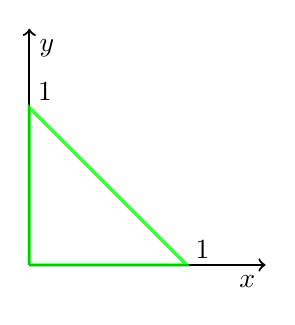
\begin{tikzpicture}[scale=2]
        %draw the main coordinate system axes
        \draw[thick,->] (0,0) -- (1.5,0) node[anchor=north east]{$x$};
        \draw[thick,->] (0,0) -- (0,1.5) node[anchor=north west]{$y$};
        
        \draw[thick, opacity=0.8, color=green, very thick] plot coordinates{(0,0) (0,1) (1,0) (0,0)};
    
        \node at (1.1,0.1) {1};
        \node at (0.1,1.1) {1};
    \end{tikzpicture}}
	\qquad\qquad
	\subfigure[]{
	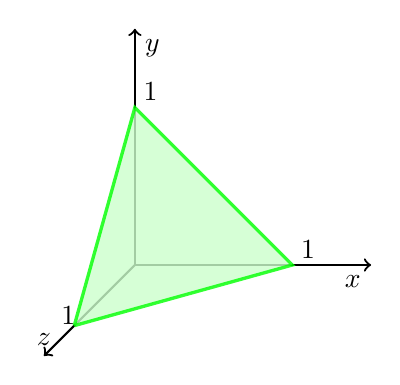
\begin{tikzpicture}[scale=2]
        %draw the main coordinate system axes
        \draw[thick,->] (0,0,0) -- (1.5,0,0) node[anchor=north east]{$x$};
        \draw[thick,->] (0,0,0) -- (0,1.5,0) node[anchor=north west]{$y$};
        \draw[thick,->] (0,0,0) -- (0,0,1.5) node[anchor=south]{$z$};
    
        \filldraw[thick, opacity=0.8, color=green!20, draw=green, very thick] plot coordinates{(0,0,1) (0,1,0) (1,0,0) (0,0,1)};
    
        \node at (1.1,0.1,0) {1};
        \node at (0.1,1.1,0) {1};
        \node at (0,0.1,1.1) {1};
	\end{tikzpicture}}
	\caption[Simplesso 2D e 3D]{A sinistra il simplesso a due dimensioni, a destra quello a tre dimensioni. Le strategie pure corrispondono ai vertici del simplesso.}
\end{figure}

\noindent Un \textbf{profilo strategico misto} è un vettore $\vec{x} = (\vec{x}_1, \dots, \vec{x}_n)$ dove la componente $\vec{x}_i$ è una strategia mista del giocatore $i \in I$. Lo \textbf{spazio delle strategie miste} è il multi-simplesso $\Theta = \prod_{i = 1}^n \Delta_i$.

Nei giochi non cooperativi si assume che le scelte dei giocatori siano indipendenti tra loro, pertanto la probabilità che un profilo strategico puro $\vec{s}$ sia usato quando viene giocato un profilo strategico misto $\vec{x}$ è data da
\begin{displaymath}
    \mathbf{\vec{x}(\vec{s})} = \prod_{i = 1}^n x_{i s_i}
\end{displaymath}
e il \textbf{payoff atteso} del giocatore $i \in I$ è
\begin{displaymath}
    u_i(\vec{x}) = \sum_{\vec{s} \in S} \vec{x}(\vec{s}) \pi_i(\vec{s})
\end{displaymath}

\section{Best replies ed equilibri di Nash}

\begin{mydef}[Best reply]
	La \defterm{best reply} di un giocatore $i \in I$ al profilo strategico $\vec{x}_{-i}$\footnote{Con $\vec{x}_{-i}$ si intende il profilo strategico misto $\vec{x} \in \Theta$ senza la componente $i$-esima.} è una strategia mista $\vec{x}_i^* \in \Delta_i$ tale per cui:
	\begin{displaymath}
		u_i(\vec{x}_i^*, \vec{x}_{-i}) \geq u_i(\vec{z}_i, \vec{x}_{-i}) \quad \forall \vec{z}_i \in \Delta_i
	\end{displaymath}
\end{mydef}
\noindent L'\textbf{insieme delle best replies} a una strategia $\vec{x}_{-i}$ per $i \in I$ si indica con $\beta_i^*(\vec{x}_{-i})$. Si noti che, escluso il caso in cui c'è un'unica miglior risposta (che è una strategia pura), il numero di best replies è infinito. Infatti:
\begin{itemize}
	\item quando il supporto di una best reply include due o più strategie pure, una loro combinazione è una best reply;
	\item se due strategie pure sono individualmente best replies, una loro combinazione è una best reply.
\end{itemize}
Il concetto di equilibrio di Nash è motivato dall'idea che una teoria di decision-making razionale non dovrebbe creare un incentivo a deviare da essa per coloro i quali ci credono.
\begin{mydef}[Equilibrio di Nash]
	Un profilo strategico $\vec{x} \in \Theta$ è un \defterm{equilibrio di Nash} se è una best reply a sè stesso, ovvero:
	\begin{displaymath}
		u_i(\vec{x}_i, \vec{x}_{-i}) \geq u_i(\vec{z}_i, \vec{x}_{-i}) \quad \forall \vec{z}_i \in \Delta_i, \forall i \in I
	\end{displaymath}
	Un equilibrio di Nash si dice \defterm{stretto} se la disuguaglianza è stretta per $\vec{z}_i \neq \vec{x}_i$.
\end{mydef}
\begin{thm}
	Un profilo strategico $\vec{x} \in \Theta$ è un equilibrio di Nash se e solo se, per ogni giocatore $i \in I$, ogni strategia pura nel supporto di $\vec{x}_i$ è una best reply a $\vec{x}_{-i}$.
\end{thm}
\noindent L'esistenza di un equilibrio di Nash è garantita dal seguente teorema.
\begin{thm}[J. Nash, 1951]
	Ogni gioco finito in forma normale ammette un equilibrio di Nash misto.
\end{thm}

\section{Teoria dei giochi evolutivi}

La \textbf{teoria dei giochi evolutivi} è una disciplina introdotta da J. M. Smith per modellare l'evoluzione del comportamento animale utilizzando mezzi e principi della teoria dei giochi. Si basa sulle seguenti assunzioni:
\begin{itemize}
	\item una popolazione grande (idealmente infinita) di individui appartenenti alla stessa specie competono per risorse disponibili in \textbf{quantità limitata};
	\item il conflitto è modellato come un gioco \textbf{simmetrico a due giocatori} selezionati in maniera casuale tra la popolazione;
	\item gli individui non giocano razionalmente, ma seguono un \textbf{pattern preprogrammato};
	\item la riproduzione è \textbf{asessuata} per cui, a meno di mutazioni, ogni nascituro sarà un clone del genitore, ovvero programmato alla sua stessa strategia;
	\item il payoff è espresso in termini di \textbf{successo riproduttivo}.
\end{itemize}
In questo framework, una strategia mista può essere interpretata in due modi matematicamente equivalenti:
\begin{itemize}
	\item ogni individuo gioca una strategia pura, ma parte della popolazione segue una strategia, il resto ne segue altre;
	\item ogni individuo gioca la stessa strategia mista.
\end{itemize}
Per trattare aspetti dinamici, la prima formulazione è la più conveniente.

\section{Strategie evolutivamente stabili}

Assumiamo che un piccolo gruppo di \textbf{invasori}, che segue una strategia $\vec{y} \in \Delta$, appaia in una popolazione che segue la strategia $\vec{x} \in \Delta$; sia $\epsilon \in (0, 1)$ la percentuale di invasori nella popolazione complessiva.

Il \textbf{payoff} in un gioco di questo tipo è lo stesso che si otterrebbe in un gioco con individui che seguono la strategia $\epsilon \vec{y} + (1 - \epsilon) \vec{x} \in \Delta$.
\begin{mydef}[Strategie evolutivamente stabili (ESS)]
	Una strategia $\vec{x} \in \Delta$ si dice \defterm{evolutivamente stabile} se per ogni $\vec{y} \in \Delta \setminus \{\vec{x}\}$ esiste $\delta \in (0, 1)$ tale per cui, per ogni $\epsilon \in (0, \delta)$, si ha
	\begin{displaymath}
		\underbrace{u(\vec{x}, \epsilon \vec{y} + (1 - \epsilon) \vec{x})}_{\text{strategia \textbf{attuale}}} > \underbrace{u(\vec{y}, \epsilon \vec{y} + (1 - \epsilon) \vec{x})}_{\text{strategia \textbf{mutante}}}
	\end{displaymath}
\end{mydef}
\begin{thm}
	Una strategia $\vec{x} \in \Delta$ è evolutivamente stabile se e solo se:
	\begin{itemize}
		\item $u(\vec{y}, \vec{x}) \leq u(\vec{x}, \vec{x})$ per ogni $\vec{y} \in \Delta$ (\defterm{equilibrio di Nash});
		\item $u(\vec{y}, \vec{x}) = u(\vec{x}, \vec{x}) \Rightarrow u(\vec{y}, \vec{y}) < u(\vec{x}, \vec{y})$ per ogni $\vec{y} \in \Delta \setminus \{\vec{x}\}$ (\defterm{condizione di stabilità}).
	\end{itemize}
\end{thm}

\noindent Dal teorema segue che:
\begin{itemize}
	\item $\Delta^{ESS} \subseteq \Delta^{NE}$, dove $\Delta^{ESS}$ e $\Delta^{NE}$ sono l'insieme delle strategie evolutivamente stabili e l'insieme degli equilibri di Nash;
	\item se $\vec{x} \in \Delta$ è un equilibro di Nash stretto, allora $\vec{x} \in \Delta^{ESS}$.
\end{itemize}
Dal punto di vista computazionale:
\begin{itemize}
	\item dire se un gioco simmetrico a due giocatori ha un ESS è NP-hard e coNP-hard;
	\item dire se $\vec{x} \in \Delta$ è ESS di un gioco simmetrico a due giocatori è coNP-hard.
\end{itemize}

\section{Dinamiche di replicazione}

Le \textbf{dinamiche di replicazione} sono una classe di sistemi dinamici utilizzati nel contesto della teoria dei giochi evolutivi per modellare la replicazione. 

Le equazioni di replicazione si distinguono rispetto ad altri modelli in quanto permettono di incorporare la distribuzione dei tipi di popolazione nella funzione di fitness, catturando così l'essenza della \textbf{selezione}. Non incorporano tuttavia le mutazioni, pertanto non sono in grado di creare nuovi tipi (strategie pure).

Sia $\vec{x}(t) \in \Delta$ il vettore che rappresenta lo \textbf{stato} della popolazione al tempo $t$, dove $x_i(t)$ è la percentuale di popolazione programmata alla strategia $i~\in~\{1, \dots, n\}$, e sia $\mat{A} = (a_{ij})$ la matrice $n \times n$ di payoff dove $a_{ij}$ è il payoff che si ottiene giocando la strategia $i$ contro un individuo che usa la strategia $j$. Il \textbf{payoff atteso} di un giocatore che segue la strategia $i$ è dato da
\begin{displaymath}
	\pi_i(\vec{x}) = (\mat{A} \vec{x})_i = \sum_j a_{ij} x_j
\end{displaymath}
mentre il \textbf{payoff medio} sull'intera popolazione è:
\begin{displaymath}
	\pi(\vec{x}) = \vec{x}^T \mat{A} \vec{x} = \sum_i x_i \pi_i(\vec{x})
\end{displaymath}
Esistono due formulazioni per le dinamiche di replicazione, una in cui il tempo scorre in maniera \textbf{continua}
\begin{displaymath}
	\frac{\dif}{\dif t} x_i(t) = x_i(t) \left(\pi_i(\vec{x}(t)) - \sum_j x_j(t) \pi_j(\vec{x}(t)) \right)
\end{displaymath}
e una in cui il tempo scorre in maniera \textbf{discreta}
\begin{displaymath}
	x_i(t + 1) = \frac{x_i(t) \pi_i(\vec{x}(t))}{\sum_j x_j(t) \pi_j(\vec{x}(t))}
\end{displaymath}
con il vincolo che $\mat{A}$ sia non negativa.\footnote{
	Esistono delle equazioni alternative per cui la convergenza è più veloce. Sia $\kappa > 0$, la formulazione continua della dinamica di replicazione diventa
	\begin{displaymath}
		\frac{\dif}{\dif t} x_i(t) = x_i(t) \left(e^{\kappa \pi_i(\vec{x}(t))} - \sum_j x_j(t) e^{\kappa \pi_j(\vec{x}(t))} \right)
	\end{displaymath}
	mentre quella discreta è:
	\begin{displaymath}
		x_i(t + 1) = \frac{x_i(t) e^{\kappa \pi_i(\vec{x}(t))}}{\sum_j x_j(t) e^{\kappa \pi_j(\vec{x}(t))}}
	\end{displaymath}
}

Si noti che il simplesso $\Delta$ è invariante rispetto entrambe le dinamiche, cioè se $\vec{x}(0) \in \Delta$ allora $\vec{x}(t) \in \Delta$ per ogni $t \geq 0$. Tipicamente la dinamica viene avviata dal baricentro di $\Delta$, ovvero $\vec{x}(0) = \vec{e} / n$.\footnote{$\vec{e}$ è un vettore di lunghezza $n$ i cui elementi sono tutti $1$.}

Un punto $\vec{x}$ si dice \textbf{stazionario} se $\frac{\dif}{\dif t} x_i(t) = 0$ per ogni $i$; si dice \textbf{asintoticamente stabile} se qualunque traiettoria avviata in un intorno sufficientemente piccolo di $\vec{x}$ converge a $\vec{x}$ per $t \rightarrow \infty$.

Il seguente teorema fornisce alcuni risultati riguardanti gli stati stazionari e stabili delle dinamiche di replicazione.
\begin{thm}[P. D. Taylor, L. B. Jonker, 1978 \& J. Nachbar, 1990]
	Un punto $\vec{x} \in \Delta$ è un equilibrio di Nash se e solo se $\vec{x}$ è il punto limite di una traiettoria di una dinamica di replicazione avviata all'interno di $\Delta$.
	
	Inoltre, se $\vec{x}$ è un ESS, allora è un punto di equilibrio asintoticamente stabile per la dinamica di replicazione.
\end{thm}

\section{Giochi doppiamente simmetrici}

Nel caso di giochi doppiamente simmetrici si possono dimostrare proprietà molto interessanti riguardanti le dinamiche di replicazione.
\begin{thm}[Teorema fondamentale della selezione naturale - V. Losert, E. Akin, 1983]
	In un gioco doppiamente simmetrico, il payoff medio della popolazione $f(\vec{x}) = \vec{x}^T \mat{A} \vec{x}$ è \defterm{strettamente crescente} lungo una qualunque traiettoria non costante di una dinamica di replicazione, ovvero per $t \geq 0$ si ha
	\begin{itemize}
		\item $\frac{\dif}{\dif t} f(\vec{x}(t)) \geq 0$ nel caso continuo;
		\item $f(\vec{x}(t + 1)) \geq f(\vec{x}(t))$ nel caso discreto;
	\end{itemize}
	con uguaglianza se e solo se $\vec{x}(t)$ è un punto stazionario.
\end{thm}
\begin{thm}[J. Hofbauer, K. Sigmund, 1988]
	In un gioco doppiamente simmetrico le seguenti affermazioni sono equivalenti:
	\begin{itemize}
		\item $\vec{x} \in \Delta^{ESS}$;
		\item $\vec{x} \in \Delta$ è un massimizzatore locale stretto di $f(\vec{x})$ in $\Delta$;
		\item $\vec{x} \in \Delta$ è un punto asintoticamente stabile nelle dinamiche di replicazione.
	\end{itemize}
\end{thm}
\noindent Inoltre $\vec{x} \in \Delta$ è un equilibrio di Nash se e solo se è un massimizzatore locale di $f(\vec{x})$ in $\Delta$.